\documentclass[11pt,a4paper]{scrreprt}
\pdfminorversion=7
\usepackage[T1]{fontenc}
\usepackage[ngerman]{babel}
\usepackage{scrhack}
\usepackage{amsmath}
\usepackage{amsfonts}
\usepackage{amssymb}
\usepackage[]{siunitx}  %% For proper units (e.g. \si{kg.m.s^{-1}}) and numbers (e.g. \num{.3e45})
%%(e.g. \num{.3e45})
\sisetup{output-decimal-marker = {,}}
\usepackage{icomma} %% entfernt das Leerzeichen hinter einem Komma in der 
%%Matheumgebung bei 3,141, aber nicht bei f(x, y)
\usepackage[pdftex]{graphicx}
\usepackage{epstopdf}
\usepackage[hidelinks]{hyperref}
\usepackage{float}
\usepackage{placeins}%% Ergmöglich \FloatBarrier
\usepackage[labelfont=bf]{caption}
\captionsetup[table]{justification=raggedright,singlelinecheck=false}

%% citation
\usepackage{url}  %% For citing webpages
%\usepackage[style=ieee,backend=biber]{biblatex}	%% Meistgenutzter Zitierstil im Ingenieurswesen
\usepackage{csquotes} %% \enquote{Text} \foreignquote{Sprache}{Text}
\usepackage[backend=biber, %% Hilfsprogramm "biber" (statt "biblatex" oder "bibtex")
style=numeric, %% Zitierstil (siehe Dokumentation)
sorting=none, %% none => choronoligisch
natbib=true, %% Bereitstellen von natbib-kompatiblen Zitierkommandos
hyperref=true, %% hyperref-Paket verwenden, um Links zu erstellen
]{biblatex}
\addbibresource{kapitel/x_literaturverzeichnis.bib}
\usepackage{acronym}
\usepackage{tabularx}
\usepackage{multirow}
\usepackage{hhline}
\usepackage{subcaption}
\usepackage{multicol} % Multi Columns für enumerations
%%%%%%%%%%%%%%%%%% Document Style
\hfuzz=2pt %% Warnung für Bad Box erst ab 2pt
\usepackage{lmodern}		%% Spezial Font
\usepackage{xcolor} 	%% farbelicher text
\usepackage[headsepline=true]{scrlayer-scrpage}
\pagestyle{scrheadings}
\lohead[]{\leftmark}	% bei odd page \lohead,\cohead und \rohead
\cohead[]{}				% bei even page \lehead,\cehead und \rehead
%\rohead[]{\rightmark} 	% bei zweiseitig \ihead, \chead \ohead
\rohead[]{{\small Super coole \LaTeX Vorlage}} 				%	HIER DEN HEADER AENDERN
\automark[section]{chapter}
%%%%%%%%%%%%%%%%% Hurenkind und Schusterjunge -> https://bfy.tw/P79K
\clubpenalty=10000
\widowpenalty=10000 
\displaywidowpenalty=10000
%%%%%%%%%%%%%%%%%
%\usepackage{blindtext}
\author{Tobias Held}
%\title{Super Cooles Thesis/ Projekt Template/ Vorlage}



\begin{document}
	\begin{titlepage}
	%\setlength{\parindent}{0pt}%Einrückung auf Titelseite verhindern
	\begin{figure}[htbp]
		
\includegraphics[height=1.4cm]{Kapitel/xx_Logo_HBRS_74mm_Pfade-eps-converted-to.pdf}
	%	\hfill
	%	
	%\includegraphics[height=1.4cm]{Kapitel/xx_BRS-Blau_Schwarz_Ohne_Hintergrund_HD.png}
	\end{figure}
 % \includegraphics[width=8cm]{Logo_HBRS_74mm_Pfade.eps}
  \linespread{1.4}%\renewcommand{\baselinestretch}{1.4}\normalsize
  \vspace{2cm}
  \begin{center}

%% einen Typ auswählen
    \begin{Huge}\textbf{Thesis}\end{Huge} \\
    \vspace{1.5cm}
%% einen Studiengang auswählen
    \begin{Large}{Master Maschinenbau - Virtuelle Produktentwicklung}\end{Large} \\
   % \begin{large}
   % 	Forschungsprojekt
   % \end{large}

    \vspace{0.7cm}
    \linespread{1.2}%\renewcommand{\baselinestretch}{1.2}\normalsize
    \begin{huge}
      \textbf{\Title}
    \end{huge}
    \linespread{1.5}%\renewcommand{\baselinestretch}{1.5}
    \normalsize
    \vspace{1cm}%{0.7cm}

    \begin{Large}{\Author \\}
    \end{Large}

    \begin{Large}% Fachbereich
        Fachbereich Elektrotechnik, Maschinenbau \\ und Technikjournalismus
    \end{Large}
  \end{center}

%  \vfill
\vspace*{\fill}

  \begin{large}
    {
      \begin{tabular}{ll}
      Name: & \Author \\
      Matrikel-Nr.: & \studentNumber \\
      Adresse: & \addressStreet \\
       & \addressZipCode \\
      Mail: & \email \\
      Erstprüferin:  & \ExaminerOne \\
      Zweitprüfer: & \ExaminerTwo \\
      Eingereicht am: & \today %\today \\ %% or type in: 01. Januar 2017
      
      \end{tabular}
	}
  \end{large}

\end{titlepage}

	%\pagestyle{empty}
\section*{Erklärung}

\Author \\
\addressStreet, \addressZipCode \\

„Ich versichere hiermit, die von mir vorgelegte Arbeit selbstständig verfasst zu haben. Alle Stellen, die wörtlich oder sinngemäß aus veröffentlichten oder nicht veröffentlichten Arbeiten anderer entnommen sind, habe ich als entnommen kenntlich gemacht. Sämtliche Quellen und Hilfsmittel, die ich für die Arbeit benutzt habe, sind angegeben. Die Arbeit hat mit gleichem Inhalt bzw. in wesentlichen Teilen noch keiner anderen Prüfungsbehörde vorgelegen.

Mir ist bewusst, dass sich die Hochschule vorbehält, meine Arbeit auf plagiierte Inhalte hin zu überprüfen und dass das Auffinden von plagiierten Inhalten zur Nichtigkeit der Arbeit, zur Aberkennung des Abschlusses und zur Exmatrikulation führen können.“
\vspace{3cm}


\noindent\parbox[t]{5cm}{\underline{\hspace{5cm}}\\\noindent Ort, Datum}%
\hfill%
\noindent\parbox[t]{5cm}{\noindent\underline{\hspace{5cm}}\\\noindent \Author}%

	\pagenumbering{Roman}
	\tableofcontents
	\listoffigures		%% Abbildungsverzeichnis || List of Figures
	\listoftables
	\newpage
\chapter*{Abkürzungsverzeichnis}
\begin{acronym}% Alphabetisch sortieren
	\acro{LCD}{liquid crystal display}
	\acro{PIN}{Persönliche Idenifikationsnummer}
	\acro{RAS}{redundant acronym syndrome}
\end{acronym}

\newpage
% Hier evtl: https://www.ctan.org/pkg/glossaries
\chapter*{Variablenverzeichnis}
\begin{table}[ht]
	\begin{tabular}{rl}
	
		\(\beta\) & Trimm: \(m\)\\		
		\(\rho\)& Wasserdichte: \(kg\cdot m^{-3}\)	\\		
		&	\\
		\(A_b\)& Blockfläche Schiff: \(m^2\)\\
		\(B_c\)& Normierte Breite: \(m\)\\
		\(Fn\) & Froude-Zahl: \(-\)\\
		\(Fn_h\) & Froude'sche Tiefenzahl: \(-\)\\	
		\(g\) & Erdbeschleunigung: \(m \cdot s^{-2}\)\\
		\(h\)& Wassertiefe: \(m\)\\
		\(H_m\)& Normierte Wassertiefe: \(m\)\\
		\(lcb\) & Schwerpunkt der Verdrängung: \(\%\)\\
		\(P_b\)& Benässte Schiffsfläche im Querschnitt: \(m\)\\
		\(P_c\)& Benässte Flussfläche im Querschnitt: \(m\)\\
		\(R\) & Widerstand: \(kN\)\\
		\(R_h\)& Hydraulischer Radius Schiff-Wasserstraße: \(m\)\\		
		
		\(u\) & Rückströmung: \(m\cdot s^{-1}\)\\
		\(W\)& Breite Wasseroberfläche: \(m\)\\
		\(w\)& Breite Flussbett: \(m\)\\
		\(S_d\) & Squat: \(m\)\\	
	 	\(z\) & Absenkung des Wasserstands: \(m\)\\
	\end{tabular}
\end{table}
	\newpage
	\pagenumbering{arabic}
	\pagestyle{scrheadings}
	
	\chapter{Einleitung}\label{ch:Einleitung}
\begin{quote}
	\glqq Mutationem motus proportionalem esse vi motrici impressae, et fieri secundum lineam rectam qua vis illa imprimitur.\grqq { }-- Sir Isaac Newton
\end{quote}
Dieses Gesetz ist besser bekannt in der Formulierung von Leonhard Euler: Kraft ist gleich Masse mal Beschleunigung. Eine Einleitung mit einem lateinischen Satz ist zwar ungewöhnlich dafür aber fast schon humorvoll. Ein packendes Zitat ist eine gute Möglichkeit für einen spannenden Start in deine Arbeit!
	\chapter{Grundlagen}\label{ch:grundlagen}
In der \texttt{00\_Beispiel.txt} sind tolle \LaTeX Beispiele, damit man nicht immer wieder googeln muss.

\section{RAS-Syndrom}\label{sec:ras-syndrom}
Akronyme sollten mit dem Befehl \texttt{$\backslash$ac} benutzt werden damit eine Verlinkung zum Verzeichnis erstellt wird, wie hier \ac{LCD} und \ac{PIN}. Viele Menschen nennen sie auch \ac{LCD}-Display oder \ac{PIN}-Nummer. Das ist RAS-Syndrom also ein \ac{RAS}-Syndrom und \ac{RAS}-Syndrome sollten vermieden werden.

\section{Stil}\label{sec:stil}
Wer ein Unterkapitel erzeugt, sollte immer mindestens ein zweites erzeugen.
	\chapter{Methodisches Vorgehen}\label{ch:methodisches_vorgehen}

	\chapter{Durchführung}\label{ch:durchfuehrung}%keine Umlaute benutzen!

	
	\chapter{Ergebnisse}\label{ch:ergebnisse}
Hier werden deine erschreckenden Erkenntnisse präsentiert.

\begin{figure}[htbp]
	\centering
	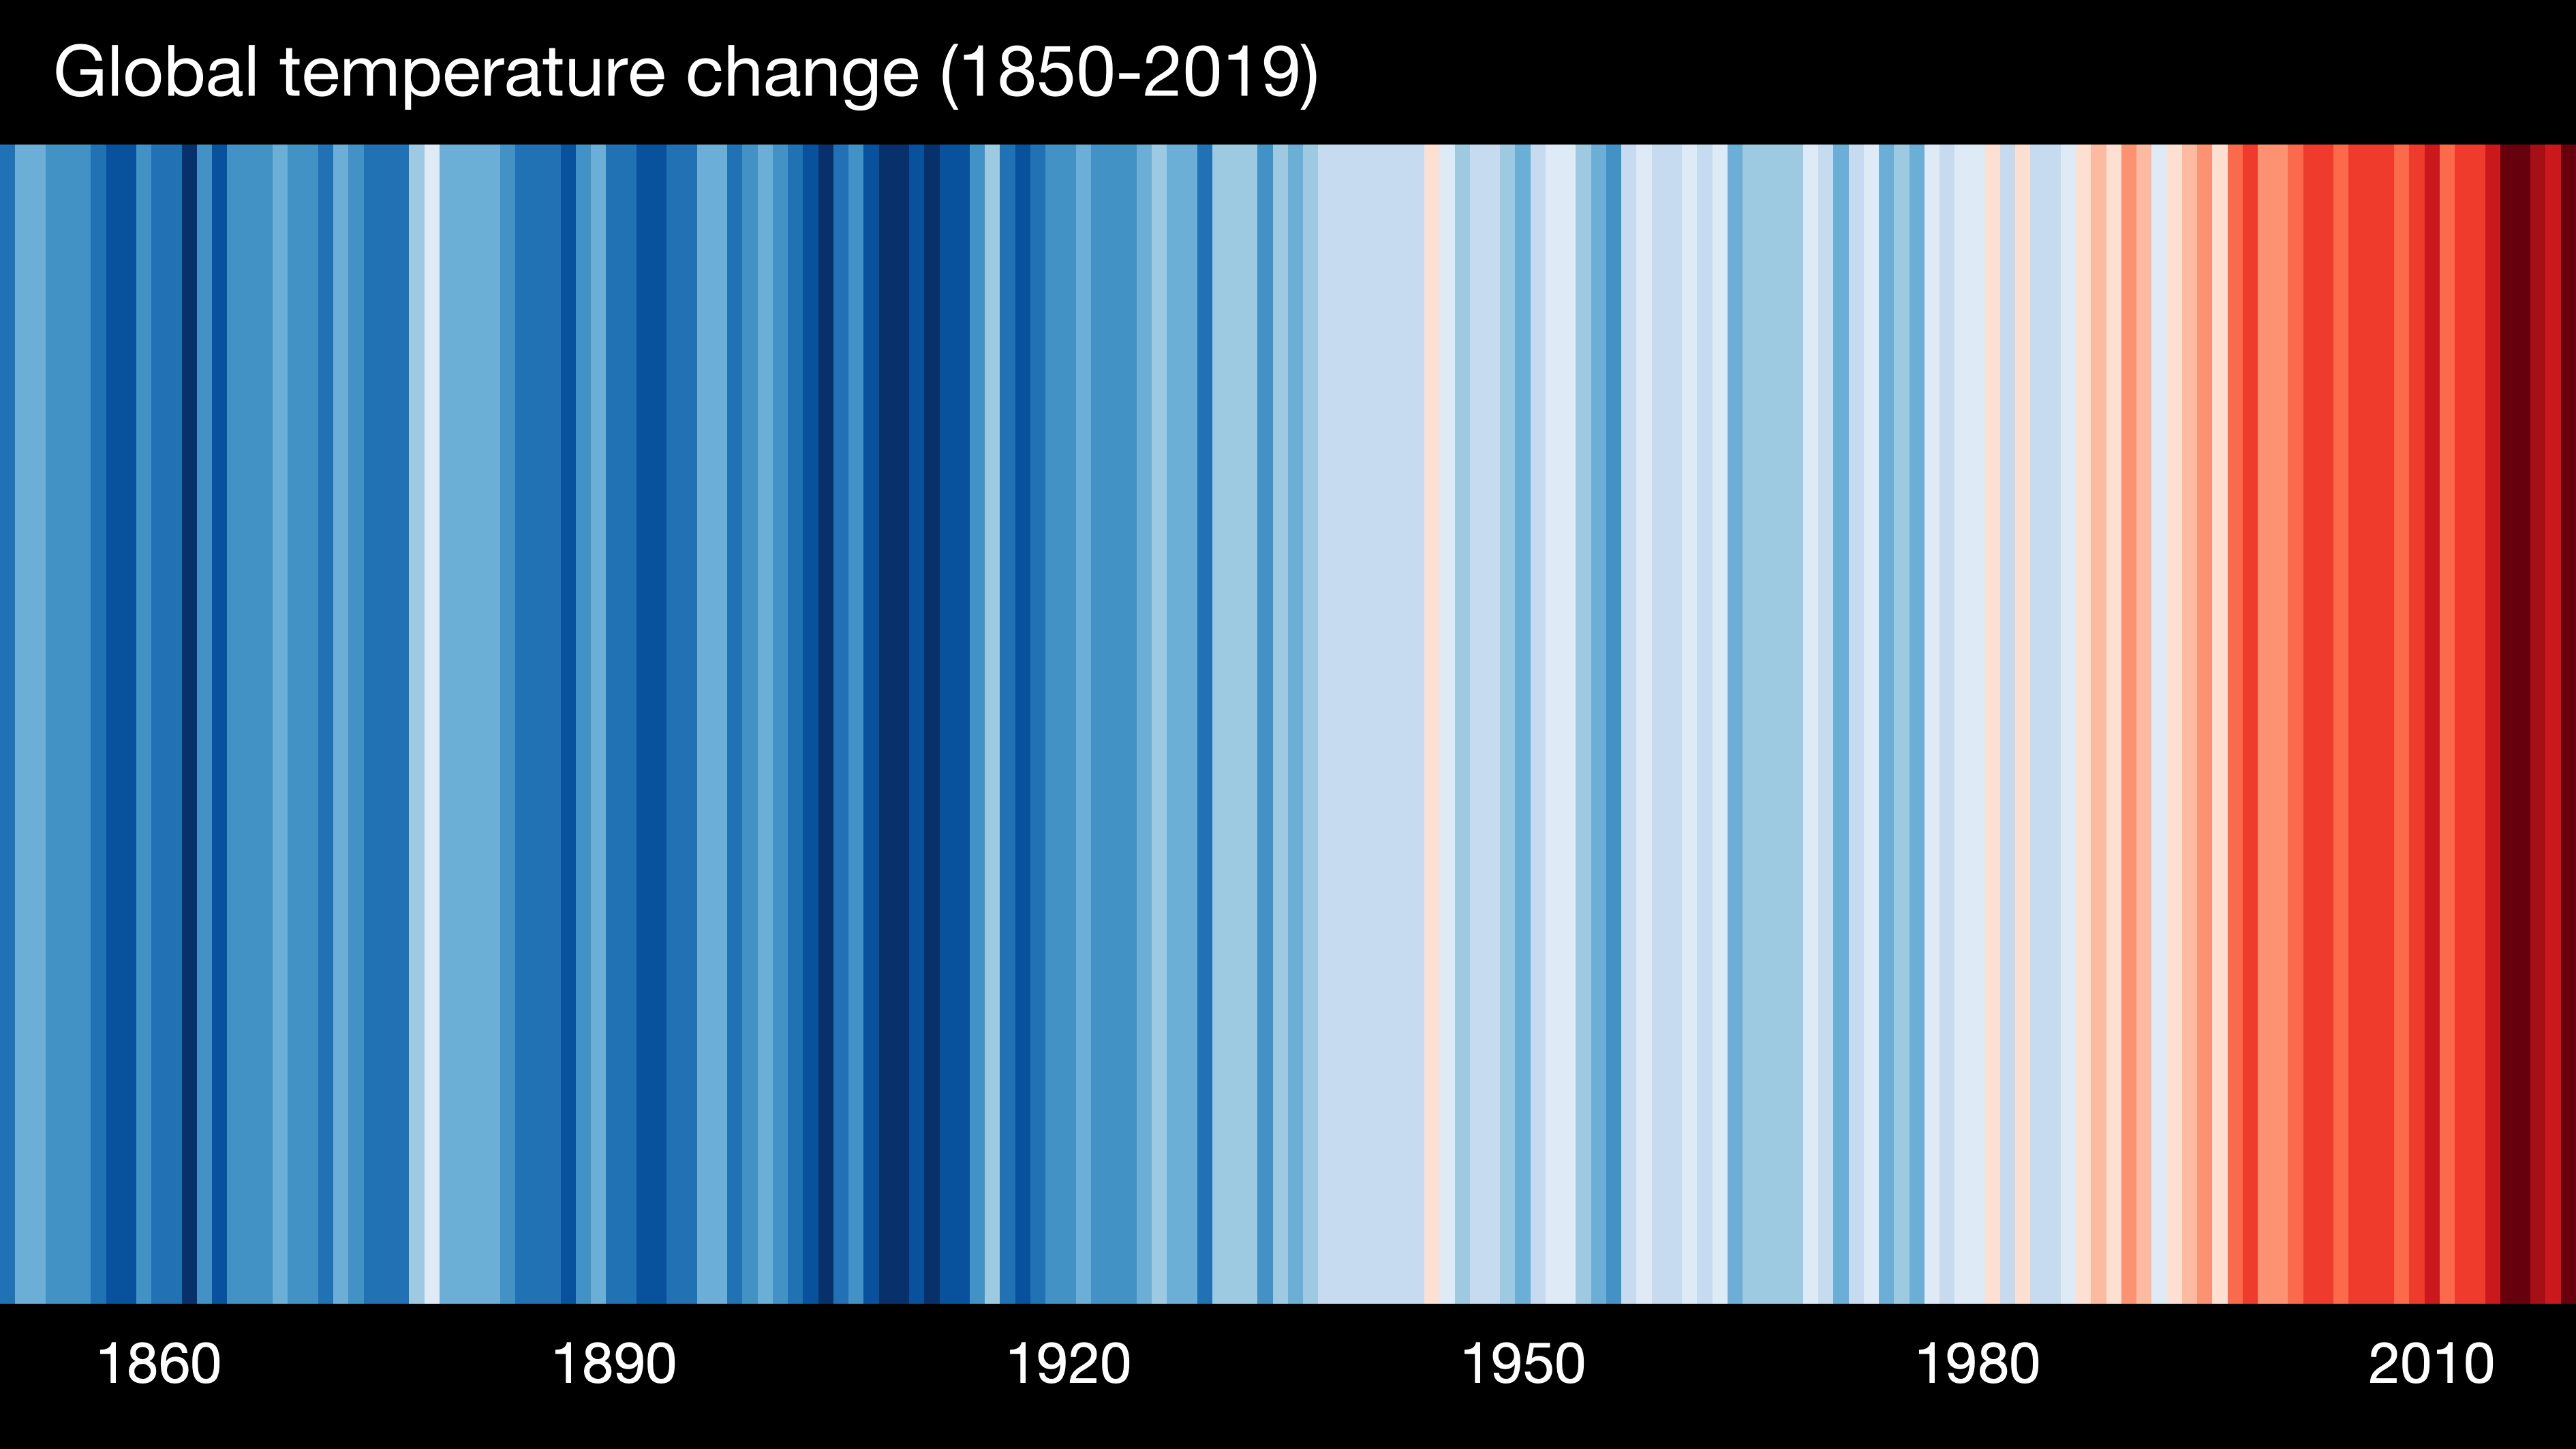
\includegraphics[width=0.9\textwidth]{figures/stripes_GLOBE---1850-2019-MO-withlabels}
	\caption[Titel der Figure]{Beschreibungstext Bla bla bla viel beschreiben sehr gut. \cite{Hawkins.2019}}
	\label{fig:DieLableIhAuhhNoo}
\end{figure}
	\chapter{Diskussion}\label{ch:diskussion}

	\chapter{Fazit und Ausblick}\label{ch:fazit_ausblick}

	
	\printbibliography
	\addcontentsline{toc}{chapter}{Literatur}
	
	
	\newpage
	\addcontentsline{toc}{chapter}{Anhang}
	\appendix
	\pagenumbering{gobble}
	\chapter*{Anhang}\label{ch:Anhang}
\chaptermark{Anhang}
%\addcontentsline{toc}{chapter}{Anhang}

\setcounter{figure}{0}
\renewcommand{\thefigure}{\Alph{section}.\arabic{figure}}
\renewcommand{\thesection}{\Alph{section}} 
\setcounter{table}{0}
\renewcommand\thetable{\Alph{section}.\arabic{table}}


\section{Warming Stripes}
\begin{figure}[htbp]
	\centering
	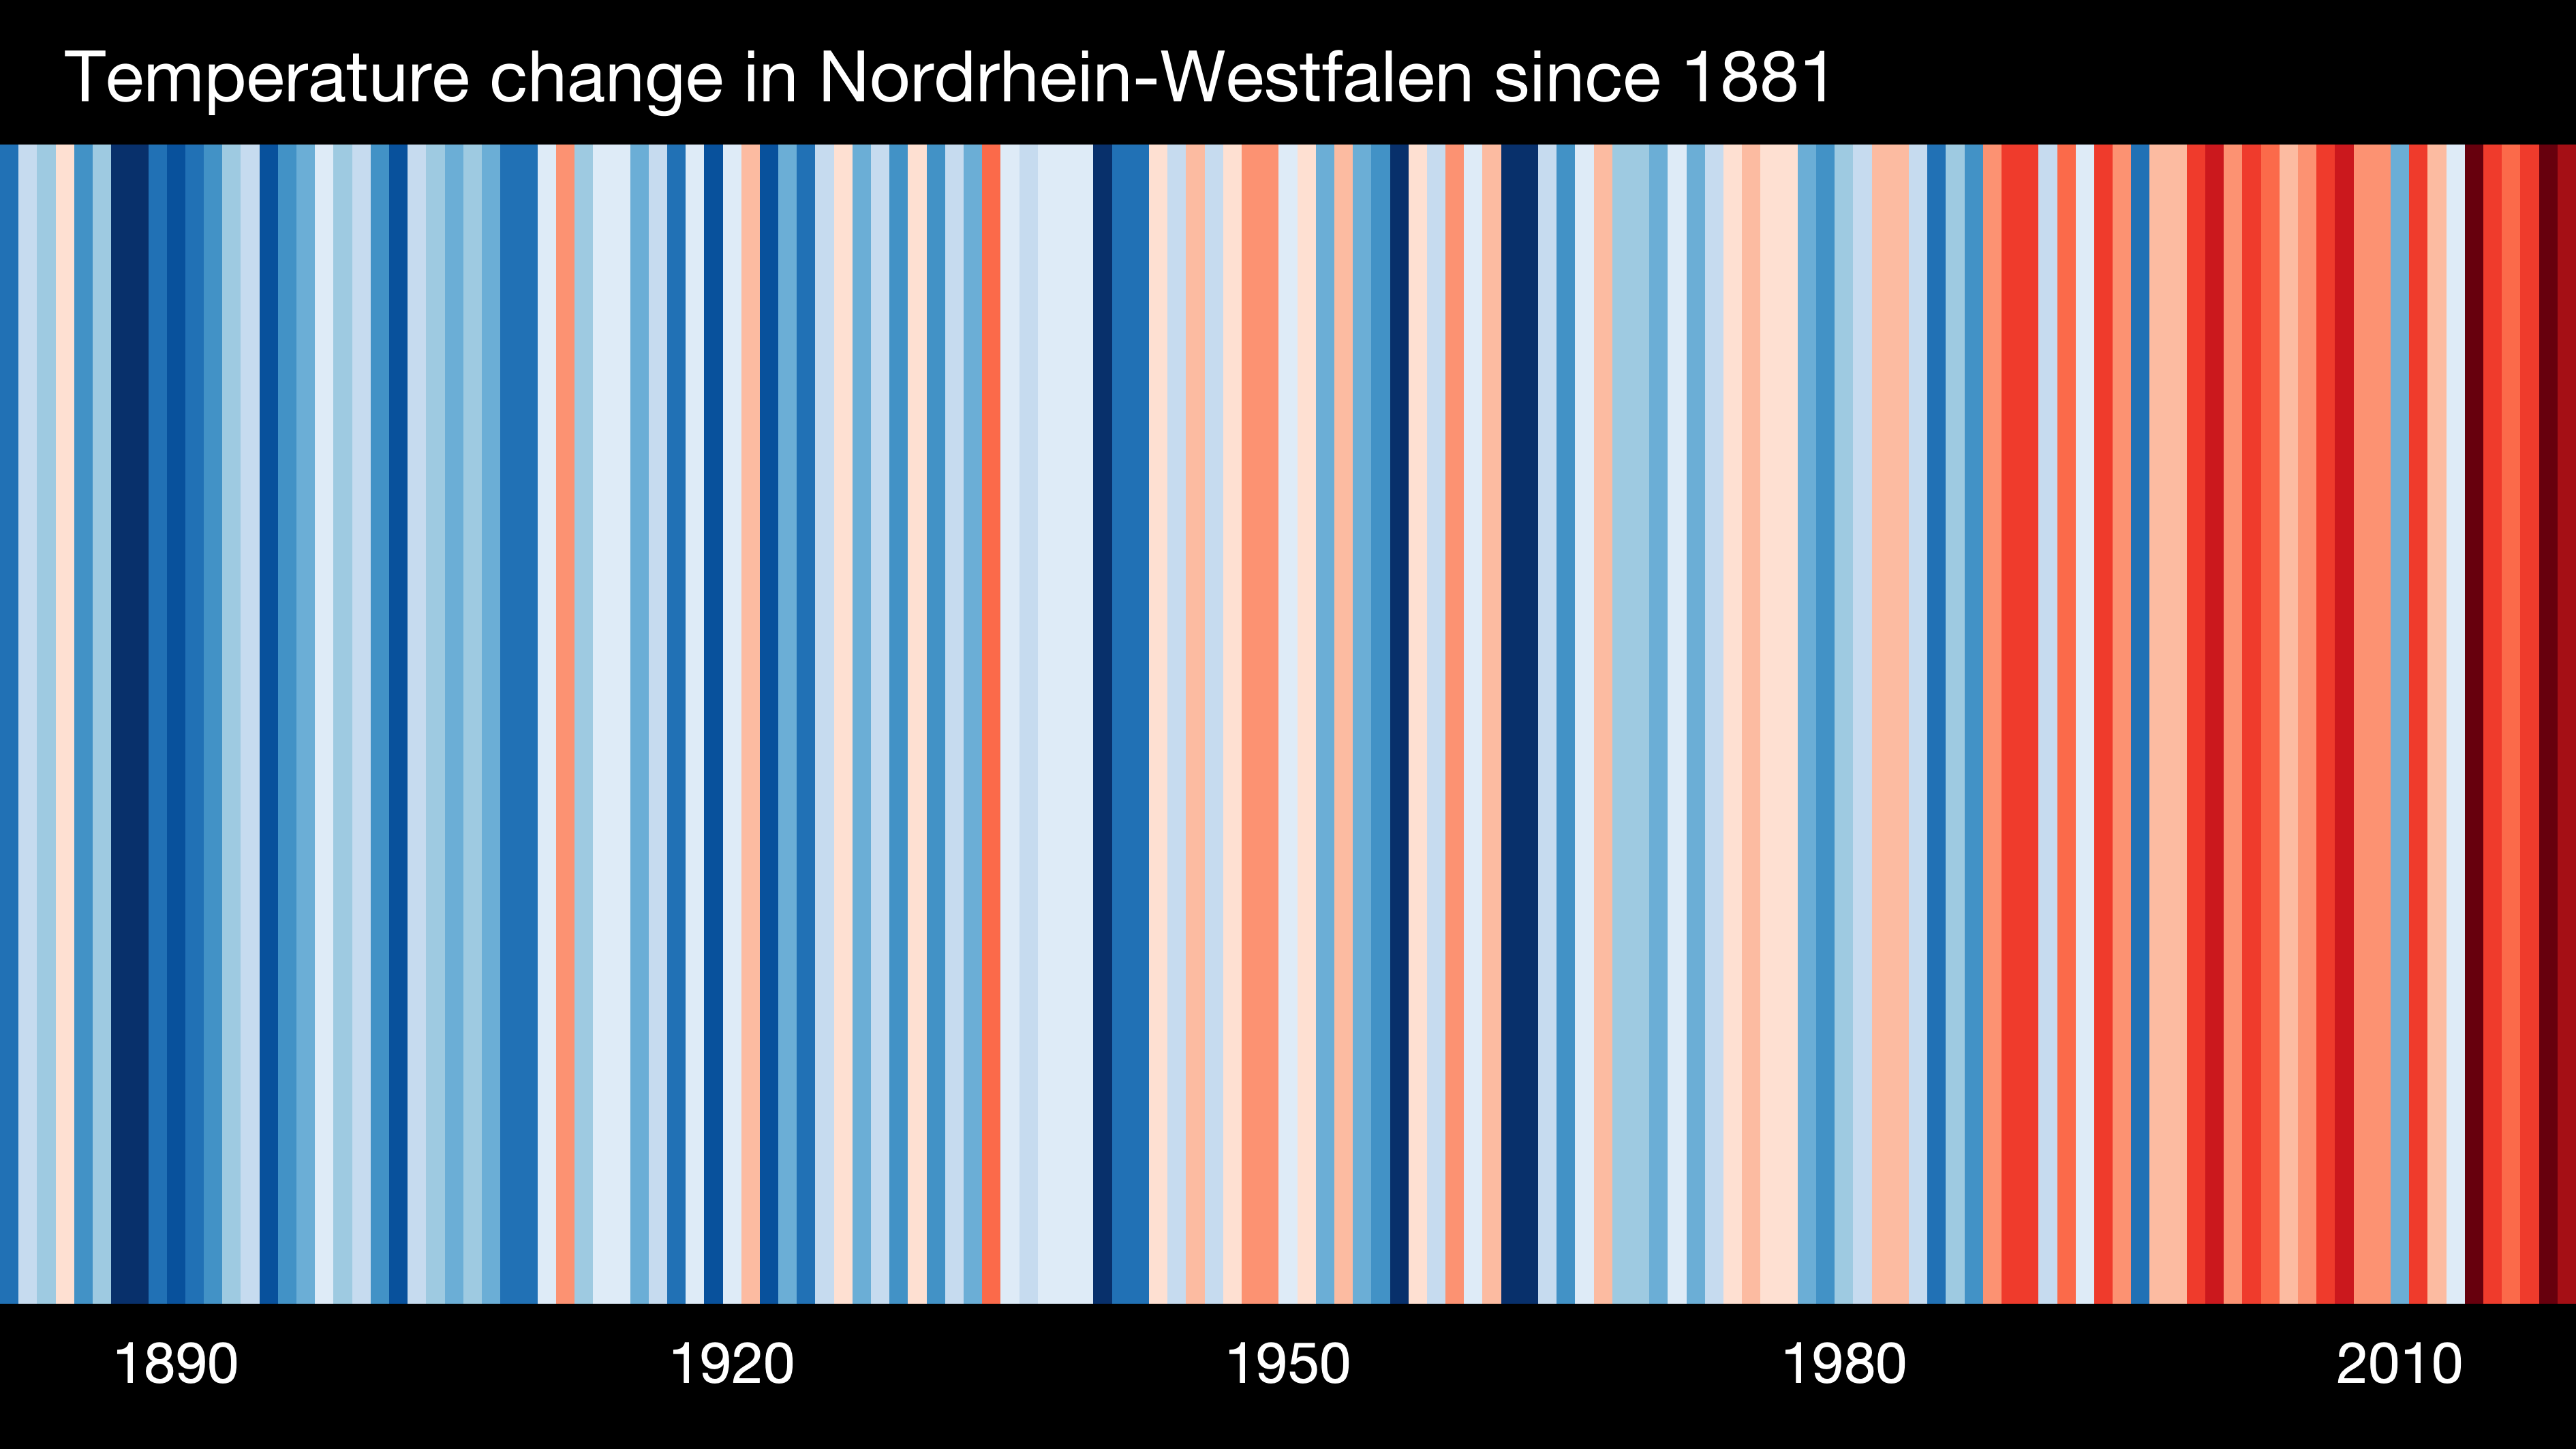
\includegraphics[width=\textwidth]{anhang/_stripes_EUROPE-Germany-Nordrhein_Westfalen-1881-2019-DW-withlabels.png}
	\caption[Titel der Figure]{Beschreibungstext Bla bla bla viel beschreiben sehr gut. \cite{Hawkins.2019}}
	\label{fig:DieLableIhAuhhNooo}
\end{figure}

	
	
\end{document}